\documentclass[a4paper,11pt, titlepage]{article}
\usepackage[MeX]{polski}
\usepackage[]{graphicx}
\usepackage[utf8]{inputenc}% ew. utf8 lub cp1250
% Zdefiniowanie autora i~tytułu:
\title{Sprawozdanie: Testy systemu transputerowego}
\author{Szymon Francuzik\and
Stanisław Jankowski}
\date{24 listopada 2008}
\frenchspacing
\begin{document}
% Wstawienie autora i~tytułu do składu:
\maketitle
\section{Opis zadania}
Problem polega na porównywaniu różnych sposobów przetwarzania zadań jednorodnych w systemie transputerowym. Zadaną architekturą systemu jest łańcuch 7 transputerów z centralnie położonym źródlem danych. Zgodnie z treścią zadania założono, iż w miarę oddalania się od źródła danych, prędkość każdego kolejnego transputera maleje dwu-, cztero- i ośmiokrotnie w stosunku do jego rzeczywistej szybkości. Rozważono następujące sposoby realizacji przetwarzania:
\begin{itemize}
\item przetwarzanie szeregowe
\item przetwarzanie równoległe z jedną fazą obliczeń i jednym przesłaniem danych - 1f1p
\item przetwarzanie równoległe z jedną fazą obliczeń i dwoma przeslaniami danych - 1f2p
\item przetwarzanie równoległe z dwoma fazami obliczeń i jednym przesłaniem danych na fazę obliczeń - 2f1p
\end{itemize}
Ponadto dla każdego z podanych wariantów rozpatrzono dwa sposoby wyboru transputerów, na których realizowane są obliczenia:
\begin{itemize}
\item wybór maksymalizujący liczbę szybkich transputerów
\begin{figure}[htp!]
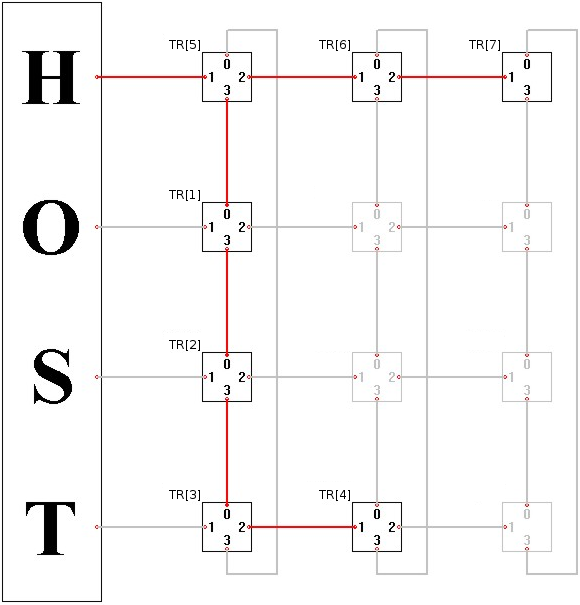
\includegraphics[scale=0.4]{proce}
\caption{Model maksymalizujący liczbę szybkich transputerów. \label{proce}}
\end{figure} 
\item wybór maksymalizujący liczbę szybkich łączy komunikacyjnych
\begin{figure}[htp!]
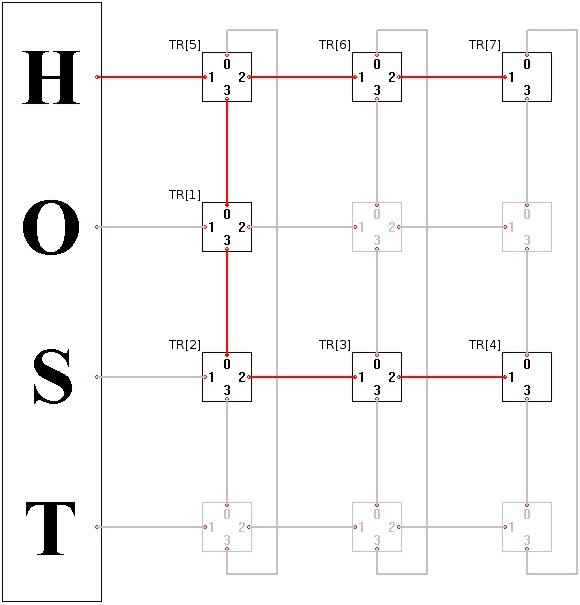
\includegraphics[scale=0.4]{lacza}
\caption{Model maksymalizujący liczbę szybkich łączy komunikacyjnych. \label{lacza}}
\end{figure} 
\end{itemize}
Wszystkie powyższe warianty rozpatrzono teoretycznie, konstruując odpowiednie problemy programowania liniowego, które pozwoliły dobrać opytmalną liczbę zadań do przetworzenia dla każdego procesora. Kryterium optymalności stanowił jak najkrótszy czas przetwarzania całej puli zadań. Aby ułożyć problemy programowania liniowego, przeprowadzono pomiary czasów komunikacji, oraz przetwarzania dla odpowiednich transputerów.

Następnie zaimplementowano warianty z przetwarzaniem 1f1p oraz 1f2p dla maksymalizacji liczby szybkich łączy oraz dla maksymalizacji liczby szybkich procesorów. Dla każdego transputera przydzielono liczbę zadań wyliczoną z modelu teoretycznego. Wyniki uzyskane z testów powyższych implementacji porównano następnie z modelami teoretycznymi.

\section{Wyznaczanie parametrow systemu}
Należało wyznaczyć czas inicjalizacji połączenia, prędkość komunikacji oraz prędkość przetwarzania pojedynczego zadania. Uwzględniono fakt, iż czas inicjalizacji połączenia oraz prędkość przetwarzania pojedynczego zadania, zależy od prędkości transputera - transputery w pierwszej kolumnie od lewej są szybsze niż pozostałe. Natomiast czas komunikacji zależny jest od rodzaju łącza - łącza poziome są szybsze niż pionowe.

\subsection{Pomiar czasów inicjalizacji połączenia, oraz prędkości komunikacji}
Napisano program mierzący czasy inicjalizacji polączeń, oraz prędkości przesyłania danych. Pomiary dokonano pomiędzy:
\begin{itemize}
\item dwoma szybkimi transputerami połączonymi wolnym łączem
\item dwoma wolnymi transputerami połączonymi szybkim lączem
\item dwoma wolnymi transputerami połączonymi wolnym lączem
\end{itemize}
Dokonano odpowiedniej synchronizacji procesów, aby upewnić się iż wszystkie one są zainicjowane i gotowe do przeprowadzenia pomiarów. Następnie uruchamiano funkcję ProcTime(), aby określić moment początku komunikacji i wysyłano pakiet danych do drugiego z transputerów, ktory natychmiast odsyłał otrzymane dane do nadawcy. Nadawca uruchamiał po raz drugi funkcję ProcTime(), aby określić moment zakończenia komunikacji. Zarowno proces nadawcy jak i odbiorcy uruchamiany był z wysokim priorytetem, co gwarantowało wysoką dokładność pomiarów.

Procedurę powtarzano dla różnych wielkości pakietów z danymi. Następnie dla otrzymanych wyników obliczono regresję liniową, dzięki której otrzymano wartości czasu inicjalizacji komunikacji, oraz prędkości komunikacji. Powyższą procedurę powtarzano dla każdej z wymienionych trzech par transputerów. Oto otrzymane wyniki czasów inicjalizacji połączeń oraz przesyłania jednego pakietu danych:
\begin{table}[h!]
\begin{tabular}{|l|l|}\hline
Typ Transputera & SetupTime[$\mu$s]\\ \hline
szybki & \textbf{10,4}\\ \hline
wolny & \textbf{10,94}\\ \hline
\end{tabular}
\caption{Wyniki pomiarów czasów inicjalizacji połączeń \label{setuptime}}
\end{table}

\begin{table}[h!]
\begin{tabular}{|l|l|}\hline
Typ Łącza & Czas[$\mu$s]\\ \hline
pionowe & 4,3\textbf{10,4}\\ \hline
poziome & 2,25\textbf{10,94}\\ \hline
\end{tabular}
\caption{Wyniki pomiarów czasów przesyłania danych \label{comunication}}
\end{table}

\subsection{Pomiar prędkości przetwarzania}
Napisano program mierzący prędkość przetwarzania pojedynczego zadania na transputerze szybkim oraz wolnym. Pojedyncze zadanie polegalo na obliczeniu metodą Hornera wartości następującego wielomianu: $W(x) = (((4*x+12)*x+3)*x+3)*x+7$.

W tym celu na każdym z dwóch tranasputerów, których dotyczyły pomiary, utworzono po dwa procesy. Proces z priorytetem niskim, na którym odbywały się obliczenia, oraz proces z priorytetem wysokim, na którym odbywały się pomiary czasu. Wybór takiego sposobu pomiarów wynika z próby jak najdokładniejszego odwzorowania architektury zastosowanej przy implementacji modeli. Po odpowiedniej synchronizacji procesów, która gwarantuje ich gotowość do przeprowadzenia pomiarów, proces obliczeniowy wysyłał sygnał - liczbę całkowitą do procesu pomiarowego i zaczynał obliczenia.  Proces pomiarowy po otrzymaniu pierwszego sygnału uruchamiał funkcję ProcTime() do uzyskania czasu rozpoczęcia obliczeń. Proces obliczeniowy po zakończeniu obliczeń wysyłał do procesu mierzącego czas kolejny sygnał. Proces mierzący, po odebraniu drugiego sygnalu, uruchamiał funkcję ProcTime() aby uzyskać czas zakończenia obliczeń. Różnica obu czasów dała czas trwania obliczeń powiększony o czas przesyłania komunikatu między procesami (ok. 18 $\mu$s). 

Procedurę powtarzano dla różnej liczby zadań do przetworzenia przez procesor, przy czym dla każdej liczby zadań pomiar przeprowadzano dwudziestokrotnie. Następnie dla otrzymanych wyników obliczono regresję liniową, dzięki ktorej otrzymano wartości prędkości obliczeń dla transputera szybkiego oraz wolnego. Oto torzymane wyniki prędkości przetwarzania pojedynczego zadania:
\begin{table}[h!]
\begin{tabular}{|l|l|}\hline
Typ Transputera & Czas[$\mu$s]\\ \hline
szybki & \textbf{6,6}\\ \hline
wolny & \textbf{6,83}\\ \hline
\end{tabular}
\caption{Wyniki pomiarów prędkości przetwarzania pojedynczego zadania \label{speedtest}}
\end{table}

\section{Opis modeli systemów}
Dla każdego wariantu realizacji obliczeń opisanego w punkcjie pierwszym, utworzono model matemetyczny. Jest nim zadanie programowania liniowego, które następnie rozwiązywano za pomocą programu lp\_solve. Pozwoliło to uzyskać optymalne rozkłady puli zadań na poszczególnych procesorach, minimalizując tym samym czasy zakończenia obliczeń.

\begin{itemize}
\item \textbf{v} - całkowita liczba zadań do realizacji przez system
\item \textbf{T} - minimalizowany całkowity czas przetwarzania v zadań
\item \textbf{li} - liczba zadań dla itego procesora, i=1..7
\item \textbf{ai} - czas przetwarzania pojedynczego zadania na itym transputerze, i=1..7
\item \textbf{s1, s2} - czas inicjalizacji komunikacji, odpowiednio dla szybkiego i wolnego transputera
\item \textbf{c1, c2} - czas przesłu jednego pakietu danych, odpowiednio wolnym i szybkim łączem
\end{itemize}
\textbf{Uwaga!
\begin{itemize}
\item Poniżej przedstawiono tylko równania i/lub ograniczenia dla wybranych modeli, bez inicjalizowania zmiennych i stałych problemu. Kompletne kody dla każdego problemu umieszczone zostały na dołączonej plycie CD. 
\item Przyjęte oznaczenia (indeksy według rysunków z rozdziału Opis zadania)
\end{itemize}
}
\subsection{Model szeregowy}
W modelu tym założono iż komunikacja między transputerami przebiega szeregowo,  to znaczy transputer - źródło przesyła dane najpierw do jednego końca łańcucha a następnie do drugiego. Dopiero po zakończeniu przesyłania danych, transputer zaczyna obliczenia. Oto problemy liniowe dla omawianego modelu, przy przyjętych oznaczeniach.(rysunek!!!)

\subsubsection{Maksymalizacja liczby szybkich procesorów}
\begin{flushleft}

minimize obj: +T;\linebreak
\linebreak
R1: T $>=$ s1+(l5+l6+l7)*c1 + s1+(l2+l3+l4)*c1 + l1*a1;\linebreak
R2: T $>=$ s1+(l5+l6+l7)*c1 + s1+(l2+l3+l4)*c1 + s1+(l3+l4)*c1 + l2*a2;\linebreak
R3: T $>=$ s1+(l5+l6+l7)*c1 + s1+(l2+l3+l4)*c1 + s1+(l3+l4)*c1 + s1+(l4)*c2 + l3*a3;\linebreak
R4: T $>=$ s1+(l5+l6+l7)*c1 + s1+(l2+l3+l4)*c1 + s1+(l3+l4)*c1 + s1+(l4)*c2 + l4*a4;\linebreak
R5: T $>=$ s1+(l5+l6+l7)*c1 + s1+(l6+l7)*c2 + l5*a5;\linebreak
R6: T $>=$ s1+(l5+l6+l7)*c1 + s1+(l6+l7)*c2 + s2+(l7)*c2 + l6*a6;\linebreak
R7: T $>=$ s1+(l5+l6+l7)*c1 + s1+(l6+l7)*c2 + s2+(l7)*c2 + l7*a7;\linebreak
R8: v $=$ l1+l2+l3+l4+l5+l6+l7;\linebreak
\end{flushleft}

Rozwiązanie problemu programowania liniowego dla tego wariantu:(tabelka!!!)
\begin{figure}[htp!]
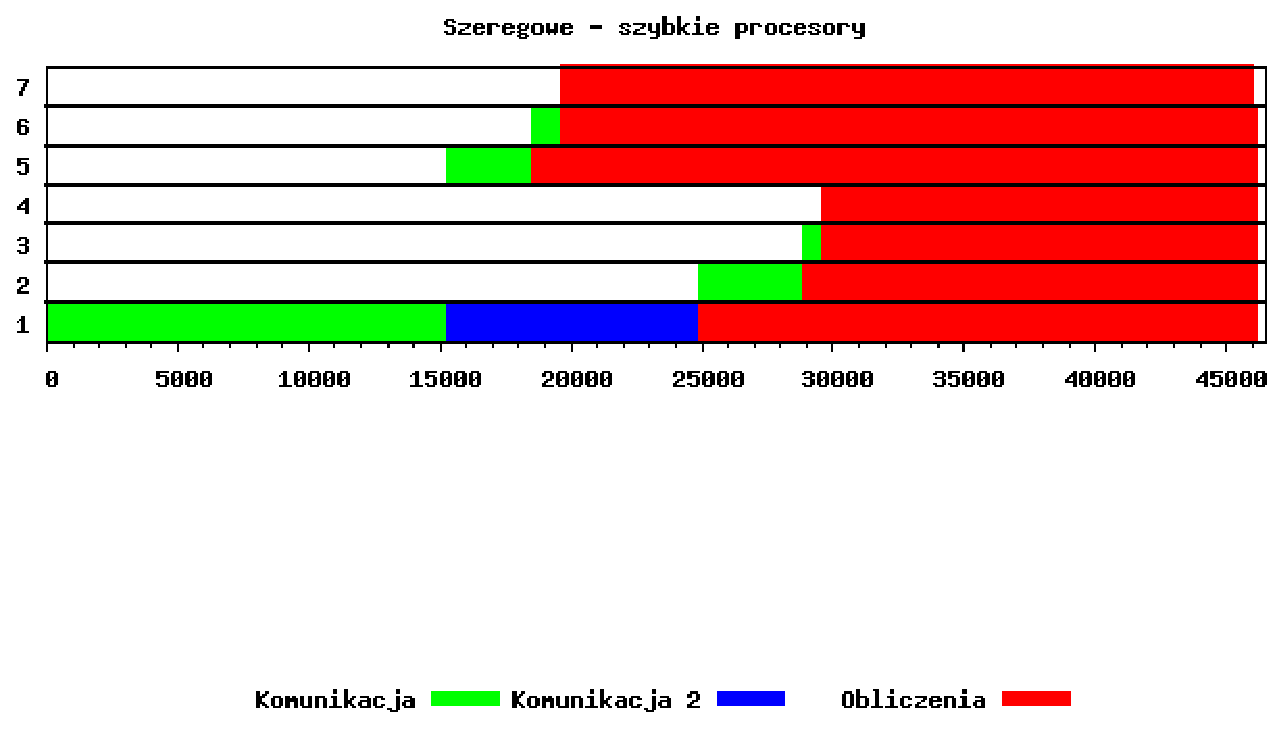
\includegraphics[width=1.0\textwidth]{wykresy/szeregowe_proc}
\caption{Diagram Gantta dla modelu szeregowego z maksymalizacją szybkich procesorów \label{szeregowe_p}}
\end{figure}

\subsubsection{Maksymalizacja liczby szybkich łączy}
\begin{flushleft}

minimize obj: +T;\linebreak
\linebreak
R1: T $>=$ s1+(l5+l6+l7)*c1 + s1+(l2+l3+l4)*c1 + l1*a1;\linebreak
R2: T $>=$ s1+(l5+l6+l7)*c1 + s1+(l2+l3+l4)*c1 + s1+(l3+l4)*c2 + l2*a2;\linebreak
R3: T $>=$ s1+(l5+l6+l7)*c1 + s1+(l2+l3+l4)*c1 + s1+(l3+l4)*c2 + s2+(l4)*c2 + l3*a3;\linebreak
R4: T $>=$ s1+(l5+l6+l7)*c1 + s1+(l2+l3+l4)*c1 + s1+(l3+l4)*c2 + s2+(l4)*c2 + l4*a4;\linebreak
R5: T $>=$ s1+(l5+l6+l7)*c1 + s1+(l6+l7)*c2 + l5*a5;\linebreak
R6: T $>=$ s1+(l5+l6+l7)*c1 + s1+(l6+l7)*c2 + s2+(l7)*c2 + l6*a6;\linebreak
R7: T $>=$ s1+(l5+l6+l7)*c1 + s1+(l6+l7)*c2 + s2+(l7)*c2 + l7*a7;\linebreak
R8: v = l1+l2+l3+l4+l5+l6+l7;\linebreak
\end{flushleft}

Rozwiązanie problemu programowania liniowego dla tego wariantu:(tabelka!!!)
\begin{figure}[h!]
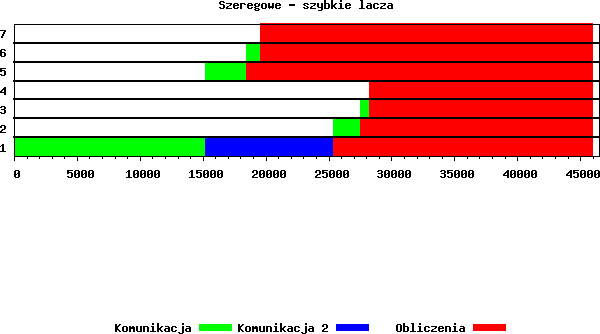
\includegraphics[width=1.0\textwidth]{wykresy/szeregowe_lacza}
\caption{Diagram Gantta dla modelu szeregowego z maksymalizacją szybkich łączy \label{szeregowe_l}}
\end{figure}

\subsection{Model 1f1p}
W modelu tym założono, że komunikacja na każdym transputerze przebiega równolegle z obliczeniami. Ponadto dla transputera-źródła równolegle odbywa się przesyłanie w obie strony. Oto problemy liniowe dla omawianego modelu, przy przyjętych oznaczeniach.(rysunek!!!)

\subsubsection{Maksymalizacja liczby szybkich procesorów}
\begin{flushleft}
minimize obj: +T;\linebreak
\linebreak
R1: T $>=$ l1*a1;\linebreak
R2: T $>=$ s1+(l2+l3+l4)*c1 +l2*a2;\linebreak
R3: T $>=$ s1+(l2+l3+l4)*c1 + s1+(l3+l4)*c1 + l3*a3;\linebreak
R4: T $>=$ s1+(l2+l3+l4)*c1 + s1+(l3+l4)*c1 + s1+(l4)*c2 +l4*a4;\linebreak
R5: T $>=$ s1+(l5+l6+l7)*c1 + l5*a5;\linebreak
R6: T $>=$ s1+(l5+l6+l7)*c1 + s1+(l5+l6)*c2 + l6*a6;\linebreak
R7: T $>=$ s1+(l5+l6+l7)*c1 + s1+(l5+l6)*c2 +  s2+(l6)*c2 + l7*a7;\linebreak
R8: v = l1+l2+l3+l4+l5+l6+l7;\linebreak
\end{flushleft}

Rozwiązanie problemu programowania liniowego dla tego wariantu:(tabelka!!!)
\begin{figure}[htp!]
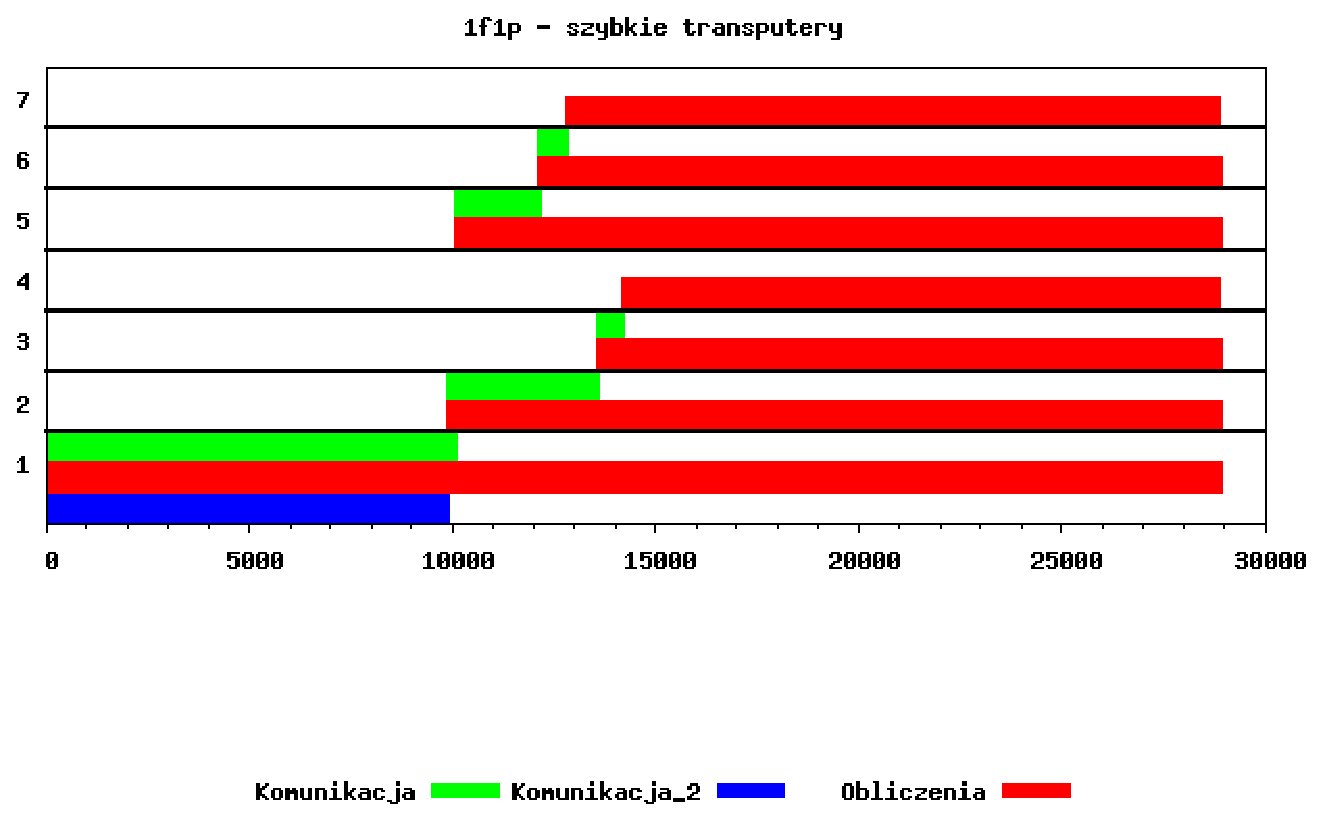
\includegraphics[width=1.0\textwidth]{wykresy/1p1f_proc}
\caption{Diagram Gantta dla modelu 1f1p z maksymalizacją szybkich procesorów \label{1p1f_p}}
\end{figure}
\subsubsection{Maksymalizacja liczby szybkich łączy}
\begin{flushleft}

minimize obj: +T;\linebreak
\linebreak
R1: T $>=$ l1*a1;\linebreak
R2: T $>=$ s1+(l2+l3+l4)*c1 + l2*a2;\linebreak
R3: T $>=$ s1+(l2+l3+l4)*c1 + s1+(l3+l4)*c2 + l3*a3;\linebreak
R4: T $>=$ s1+(l2+l3+l4)*c1 + s1+(l3+l4)*c2 + s2+(l4)*c2 +l4*a4;\linebreak
R5: T $>=$ s1+(l5+l6+l7)*c1 + l5*a5;\linebreak
R6: T $>=$ s1+(l5+l6+l7)*c1 + s1+(l5+l6)*c2 + l6*a6;\linebreak
R7: T $>=$ s1+(l5+l6+l7)*c1 + s1+(l5+l6)*c2 +  s2+(l6)*c2 + l7*a7;\linebreak
R8: v = l1+l2+l3+l4+l5+l6+l7;\linebreak
\end{flushleft}

Rozwiązanie problemu programowania liniowego dla tego wariantu:(tabelka!!!)
\begin{figure}[htp!]
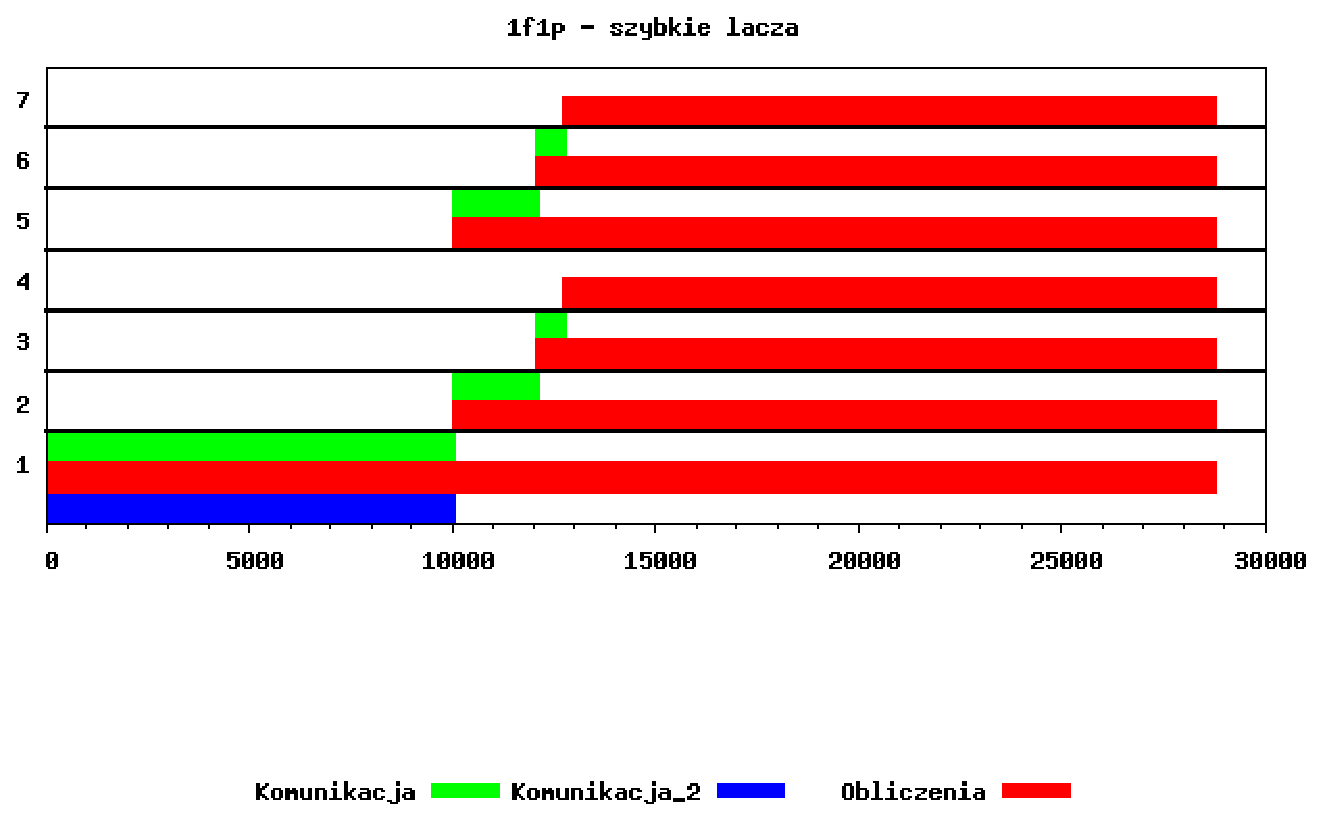
\includegraphics[width=1.0\textwidth]{wykresy/1p1f_lacza}
\caption{Diagram Gantta dla modelu 1f1p z maksymalizacją szybkich łączy \label{1p1f_l}}
\end{figure}
\subsection{Model 1f2p}
W modelu tym założono, że komunikacja odbywa się w dwóch etapach. W pierwszym etapie komunikacji, transputer odbiorca otrzymuje dane potrzebne mu do całkowitej realizacji swojej części obliczeń. W drugim etapie komunikacji otrzymuje natomiast dane do przesłania kolejnym transputerom w łańcuchu. Proces obliczeń i komunikacji został zrównoleglony w maksymalnym możliwym stopniu. Oto problemy liniowe dla omawianego modelu, przy przyjętych oznaczeniach.(rysunek!!!)

\subsubsection{Maksymalizacja liczby szybkich procesorów}
\begin{flushleft}

minimize obj: +T;\linebreak
\linebreak
R1: T $>=$ l1*a1;\linebreak
R2: T $>=$ s1+(l2)*c1 + l2*a2;\linebreak
R3: T $>=$ s1+(l2)*c1 + s1+(l3+l4)*c1 + s1+(l3)*c1 + l3*a3;\linebreak
R4: T $>=$ s1+(l2)*c1 + s1+(l3+l4)*c1 + s1+(l3)*c1 + s1+(l4)*c1 + s1+(l4)*c2 + l4*a4;\linebreak
R5: T $>=$ s1+(l5)*c1 + l5*a5;\linebreak
R6: T $>=$ s1+(l5)*c1 + s1+(l6+l7)*c1 + s1+(l6)*c2 + l6*a6;\linebreak
R7: T $>=$ s1+(l5)*c1 + s1+(l6+l7)*c1 + s1+(l6)*c2 + s1*(l7)*c2 + s2*(l7)*c2 +l7*a7;\linebreak
R8: v = l1+l2+l3+l4+l5+l6+l7;\linebreak
\end{flushleft}

Rozwiązanie problemu programowania liniowego dla tego wariantu:(tabelka!!!)
\begin{figure}[htp!]
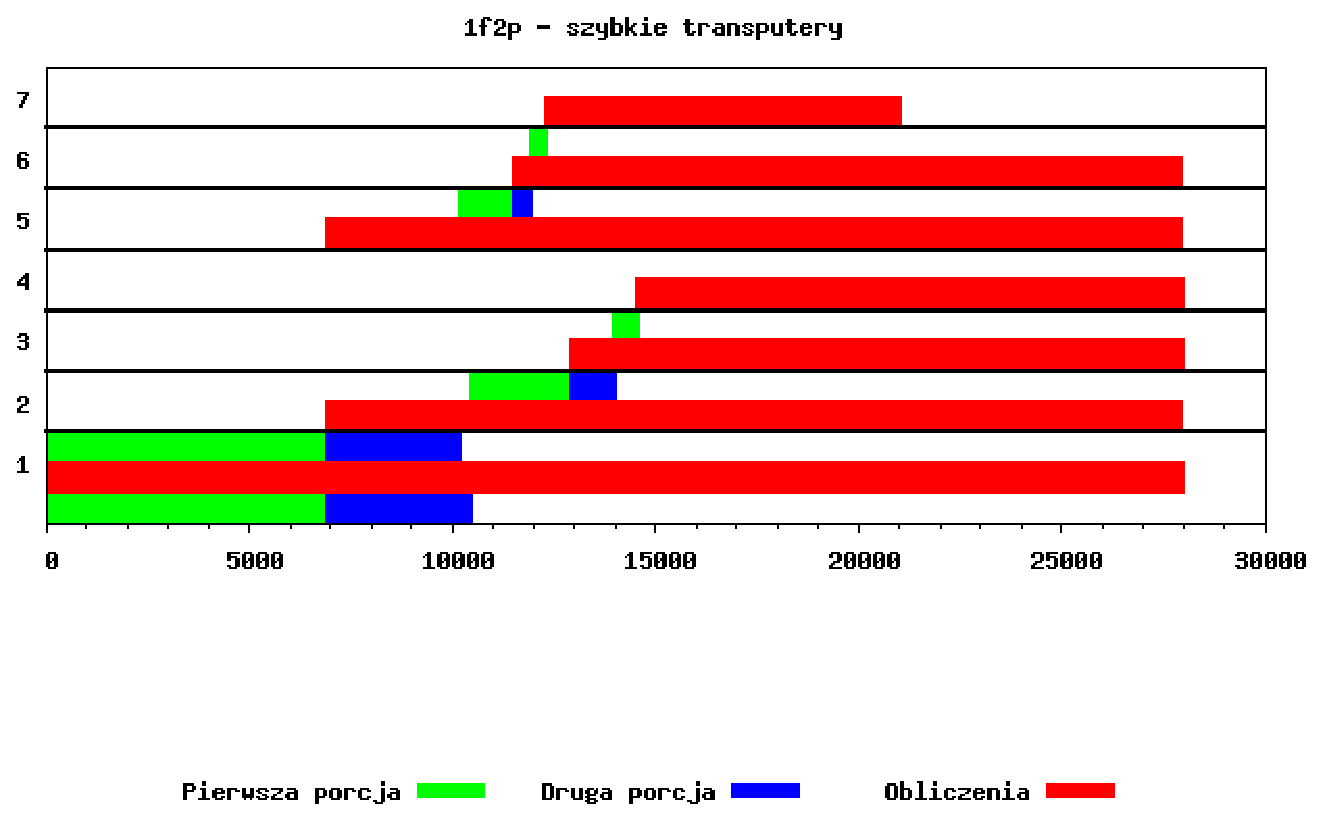
\includegraphics[width=1.0\textwidth]{wykresy/2p1f_proc}
\caption{Diagram Gantta dla modelu 1f2p z maksymalizacją szybkich procesorów \label{2p1f_p}}
\end{figure}

\subsubsection{Maksymalizacja liczby szybkich łączy}
\begin{flushleft}

minimize obj: +T;\linebreak
\linebreak
R1: T $>=4$ l1*a1;\linebreak
R2: T $>=$ s1+(l2)*c1 + l2*a2;\linebreak
R3: T $>=$ s1+(l2)*c1 + s1+(l3+l4)*c1 + s1+(l3)*c2 + l3*a3;\linebreak
R4: T $>=$ s1+(l2)*c1 + s1+(l3+l4)*c1 + s1+(l3)*c2 + s1+(l4)*c2 + s2+(l4)*c2 + l4*a4;\linebreak
R5: T $>=$ s1+(l5)*c1 + l5*a5;\linebreak
R6: T $>=$ s1+(l5)*c1 + s1+(l6+l7)*c1 + s1+(l6)*c2 + l6*a6;\linebreak
R7: T $>=$ s1+(l5)*c1 + s1+(l6+l7)*c1 + s1+(l6)*c2 + s1*(l7)*c2 + s2*(l7)*c2 + l7*a7;\linebreak
R8: v = l1+l2+l3+l4+l5+l6+l7;\linebreak
\end{flushleft}

Rozwiązanie problemu programowania liniowego dla tego wariantu:(tabelka!!!)
\begin{figure}[htp!]
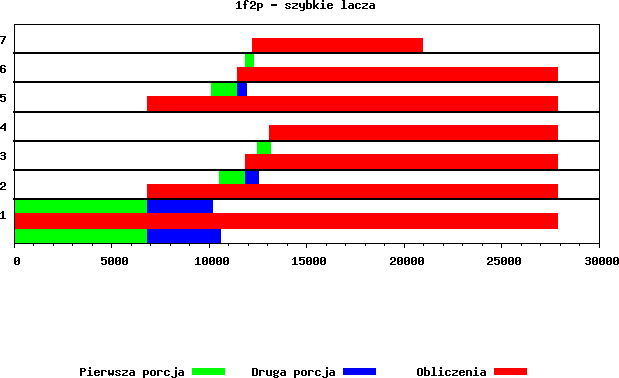
\includegraphics[width=1.0\textwidth]{wykresy/2p1f_lacza}
\caption{Diagram Gantta dla modelu 1f2p z maksymalizacją szybkich łączy \label{2p1f_l}}
\end{figure}

\subsection{Model 2f1p}końców
W modelu tym komunikację między transputerami rozbito na dwie fazy. W pierwszej, każdy z transputerów otrzymuje tylko częśc potrzebnych mu do obliczeń danych i może wykonać pierwszę fazę obliczeń. Natomiast w drugiej fazie komunikacji każdy z transputerów otrzymiuje drugą część potrzebnych mu do obliczeń danych. Przesyłanie i obliczenia realizowane sę w maksymalnie zrównoleglony sposob. 
Do opisu powyższego modelu niezbędne bylo wprowadzenie nowych parametrów opisujących system:
\begin{itemize}
\item \textbf{ob}ij - Początek obliczeń na itym transputerze w jotej fazie, i=1..7, j=1..2, wyjątek dla pierwszego transputera - ob1
\item \textbf{oe}ij - Koniec obliczeń na itym transputerze w jotej fazie, i=1..7, j=1..2, wyjątek dla pierwszego transputera - oe1
\item \textbf{kb}ij - Początek komunikacji na itym transputerze w jotej fazie, i=1..6, j=1..2, wyjątek dla pierwszego transputera - kbijl, gdzie l oznacza: g - komunikację w stronę węzła 7, d - w stronę węzła 4
\item \textbf{ke}ij - Koniec komunikacji na itym transputerze w jotej fazie, i=1..6, j=1..2, wyjątek dla pierwszego transputera - keijl, gdzie l oznacza: g - komunikację w stronę węzła 7, d - w stronę węzła 4 
\end{itemize}
Oto problemy liniowe dla omawianego modelu, przy przyjętych oznaczeniach.(rysunek!!!)
\subsubsection{Maksymalizacja liczby szybkich procesorów}

\begin{flushleft}
minimize obj: T;\linebreak
\linebreak
r1: T $>=$ oe1;\linebreak
r2: T $>=$ oe22;\linebreak
r3: T $>=$ oe32;\linebreak
r4: T $>=$ oe42;\linebreak
r5: T $>=$ oe52;\linebreak
r6: T $>=$ oe62;\linebreak
r7: T $>=$ oe72;\linebreak 
\linebreak
r8: kb21 $>=$ ke11d;\linebreak
r9: kb22 $>=$ ke12d;\linebreak
r10: kb31 $>=$ ke21;\linebreak
r11: kb32 $>=$ ke22;\linebreak
r12: kb41 $>=$ ke31;\linebreak
r13: kb42 $>=$ ke32;\linebreak
r14: kb51 $>=$ ke11g;\linebreak
r15: kb52 $>=$ ke12g;\linebreak
r16: kb61 $>=$ ke51;\linebreak
r17: kb62 $>=$ ke52;\linebreak
\linebreak
r18: v = l1 + l21 + l22 + l31 + l32 + l41 + l42 + l51 + l52 + l61 + l62 + l71 + l72;\linebreak
\linebreak
r19: ke11g = kb11g + s1+(l51+l61+l71)*c1;\linebreak
r20: ke12g = kb12g + s1+(l52+l62+l72)*c1;\linebreak
r21: ke11d = kb11d + s1+(l21+l31+l41)*c1;\linebreak
r22: ke12d = kb12d + s1+(l22+l32+l42)*c1;\linebreak
r23: ke21 = kb21 + s1+(l31+l41)*c1;\linebreak
r24: ke22 = kb22 + s1+(l32+l42)*c1;\linebreak
r25: ke31 = kb31 + s1+(l41)*c2;\linebreak
r26: ke32 = kb32 + s1+(l42)*c2;\linebreak
r27: ke51 = kb51 + s1+(l61+l71)*c2;\linebreak
r28: ke52 = kb52 + s1+(l62+l72)*c2;\linebreak
r29: ke61 = kb61 + s2+(l71)*c2;\linebreak
r30: ke62 = kb62 + s2+(l72)*c2;\linebreak
\linebreak
r31: kb12g $>=$ ke11g;\linebreak
r32: kb12d $>=$ ke11d;\linebreak
r33: kb22 $>=$ ke21;\linebreak
r34: kb32 $>=$ ke31;\linebreak
r35: kb42 $>=$ ke41;\linebreak
r36: kb52 $>=$ ke51;\linebreak
r37: kb62 $>=$ ke61;\linebreak
\linebreak
r38: ob22 $>=$ oe21;\linebreak
r39: ob32 $>=$ oe31;\linebreak
r40: ob42 $>=$ oe41;\linebreak
r41: ob52 $>=$ oe51;\linebreak
r42: ob62 $>=$ oe61;\linebreak
r43: ob72 $>=$ oe71;\linebreak
\linebreak
r44: ob21 $>=$ ke11d;\linebreak
r45: ob22 $>=$ ke12d;\linebreak
r46: ob31 $>=$ ke21;\linebreak
r47: ob32 $>=$ ke22;\linebreak
r48: ob41 $>=$ ke31;\linebreak
r49: ob42 $>=$ ke32;\linebreak
r50: ob51 $>=$ ke11g;\linebreak
r51: ob52 $>=$ ke12g;\linebreak
r52: ob61 $>=$ ke51;\linebreak
r53: ob62 $>=$ ke52;\linebreak
r54: ob71 $>=$ ke61;\linebreak
r55: ob72 $>=$ ke62;\linebreak
\linebreak
r56: oe1 = ob1 + a1*l1;\linebreak
r57: oe21 = ob21 + a2*l21;\linebreak
r58: oe22 = ob22 + a2*l22;\linebreak
r59: oe31 = ob31 + a3*l31;\linebreak
r60: oe32 = ob32 + a3*l32;\linebreak
r61: oe41 = ob41 + a4*l41;\linebreak
r62: oe42 = ob42 + a4*l42;\linebreak
r63: oe51 = ob51 + a5*l51;\linebreak
r64: oe52 = ob52 + a5*l52;\linebreak
r65: oe61 = ob61 + a6*l61;\linebreak
r66: oe62 = ob62 + a6*l62;\linebreak
r67: oe71 = ob71 + a7*l71;\linebreak
r68: oe72 = ob72 + a7*l72;\linebreak
\end{flushleft}

Rozwiązanie problemu programowania liniowego dla tego wariantu:(tabelka!!!)
\begin{figure}[htp!]
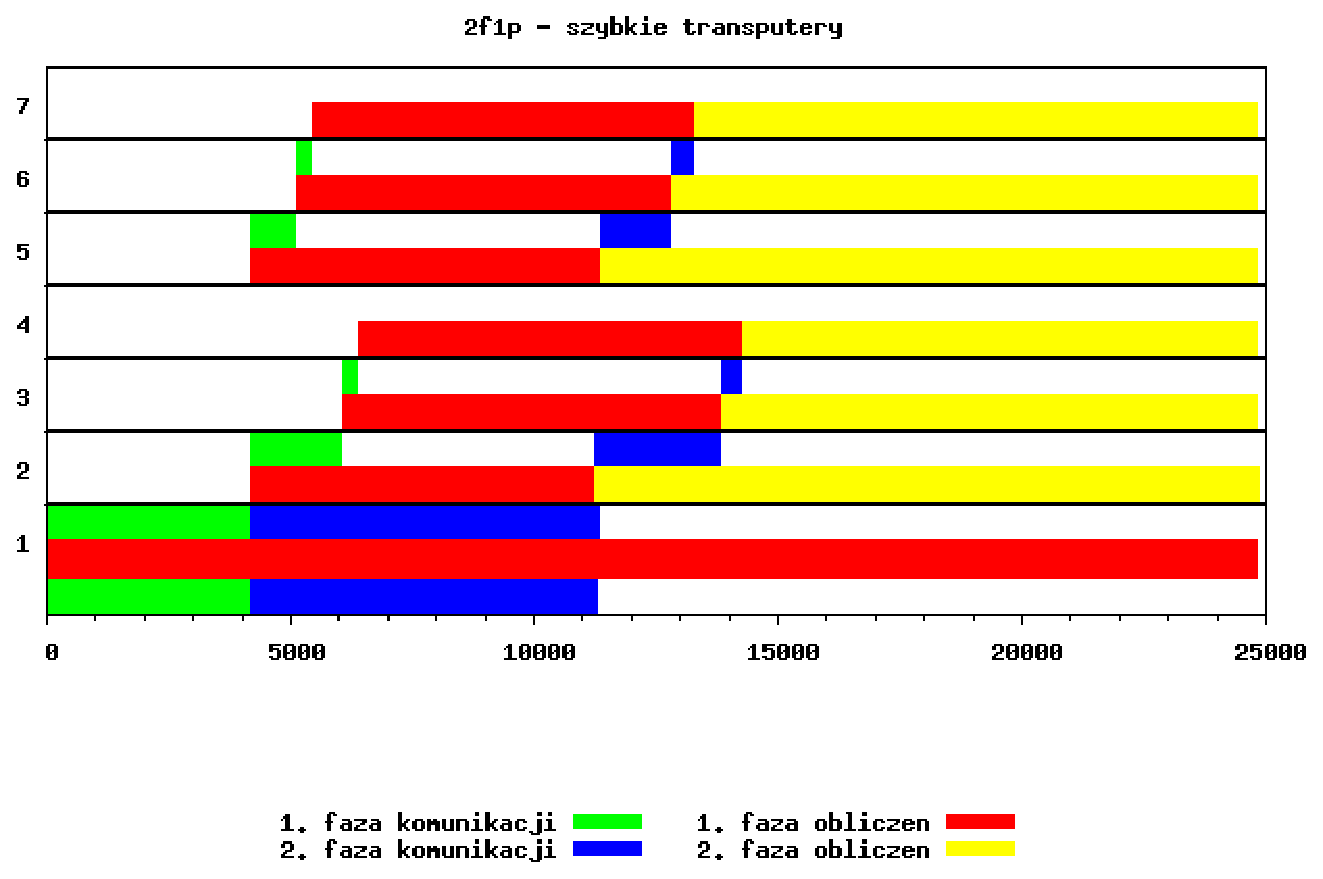
\includegraphics[width=1.0\textwidth]{wykresy/1p2f_proc}
\caption{Diagram Gantta dla modelu 2f1p z maksymalizacją szybkich procesorów \label{1p2f_p}}
\end{figure}

\subsubsection{Maksymalizacja liczby szybkich łączy}

\begin{flushleft}
minimize obj: T;\linebreak
\linebreak
r1: T $>=$ oe1;\linebreak
r2: T $>=$ oe22;\linebreak
r3: T $>=$ oe32;\linebreak
r4: T $>=$ oe42;\linebreak
r5: T $>=$ oe52;\linebreak
r6: T $>=$ oe62;\linebreak
r7: T $>=$ oe72;\linebreak
\linebreak
r8: kb21 $>=$ ke11d;\linebreak
r9: kb22 $>=$ ke12d;\linebreak
r10: kb31 $>=$ ke21;\linebreak
r11: kb32 $>=$ ke22;\linebreak
r12: kb41 $>=$ ke31;\linebreak
r13: kb42 $>=$ ke32;\linebreak
r14: kb51 $>=$ ke11g;\linebreak
r15: kb52 $>=$ ke12g;\linebreak
r16: kb61 $>=$ ke51;\linebreak
r17: kb62 $>=$ ke52;\linebreak
\linebreak
r18: v = l1 + l21 + l22 + l31 + l32 + l41 + l42 + l51 + l52 + l61 + l62 + l71 + l72;\linebreak
\linebreak
r19: ke11g = kb11g + s1+(l51+l61+l71)*c1;\linebreak
r20: ke12g = kb12g + s1+(l52+l62+l72)*c1;\linebreak
r21: ke11d = kb11d + s1+(l21+l31+l41)*c1;\linebreak
r22: ke12d = kb12d + s1+(l22+l32+l42)*c1;\linebreak
r23: ke21 = kb21 + s1+(l31+l41)*c2;\linebreak
r24: ke22 = kb22 + s1+(l32+l42)*c2;\linebreak
r25: ke31 = kb31 + s2+(l41)*c2;\linebreak
r26: ke32 = kb32 + s2+(l42)*c2;\linebreak
r27: ke51 = kb51 + s1+(l61+l71)*c2;\linebreak
r28: ke52 = kb52 + s1+(l62+l72)*c2;\linebreak
r29: ke61 = kb61 + s2+(l71)*c2;\linebreak
r30: ke62 = kb62 + s2+(l72)*c2;\linebreak
\linebreak
r31: kb12g $>=$ ke11g;\linebreak
r32: kb12d $>=$ ke11d;\linebreak
r33: kb22 $>=$ ke21;\linebreak
r34: kb32 $>=$ ke31;\linebreak
r35: kb42 $>=$ ke41;\linebreak
r36: kb52 $>=$ ke51;\linebreak
r37: kb62 $>=$ ke61;\linebreak
\linebreak
r38: ob22 $>=$ oe21;\linebreak
r39: ob32 $>=$ oe31;\linebreak
r40: ob42 $>=$ oe41;\linebreak
r41: ob52 $>=$ oe51;\linebreak
r42: ob62 $>=$ oe61;\linebreak
r43: ob72 $>=$ oe71;\linebreak
\linebreak
r44: ob21 $>=$ ke11d;\linebreak
r45: ob22 $>=$ ke12d;\linebreak
r46: ob31 $>=$ ke21;\linebreak
r47: ob32 $>=$ ke22;\linebreak
r48: ob41 $>=$ ke31;\linebreak
r49: ob42 $>=$ ke32;\linebreak
r50: ob51 $>=$ ke11g;\linebreak
r51: ob52 $>=$ ke12g;\linebreak
r52: ob61 $>=$ ke51;\linebreak
r53: ob62 $>=$ ke52;\linebreak
r54: ob71 $>=$ ke61;\linebreak
r55: ob72 $>=$ ke62;\linebreak
\linebreak
r56: oe1 = ob1 + a1*l1;\linebreak
r57: oe21 = ob21 + a2*l21;\linebreak
r58: oe22 = ob22 + a2*l22;\linebreak
r59: oe31 = ob31 + a3*l31;\linebreak
r60: oe32 = ob32 + a3*l32;\linebreak
r61: oe41 = ob41 + a4*l41;\linebreak
r62: oe42 = ob42 + a4*l42;\linebreak
r63: oe51 = ob51 + a5*l51;\linebreak
r64: oe52 = ob52 + a5*l52;\linebreak
r65: oe61 = ob61 + a6*l61;\linebreak
r66: oe62 = ob62 + a6*l62;\linebreak
r67: oe71 = ob71 + a7*l71;\linebreak
r68: oe72 = ob72 + a7*l72;\linebreak
\end{flushleft}

Rozwiązanie problemu programowania liniowego dla tego wariantu:(tabelka!!!)
\begin{figure}[htp!]
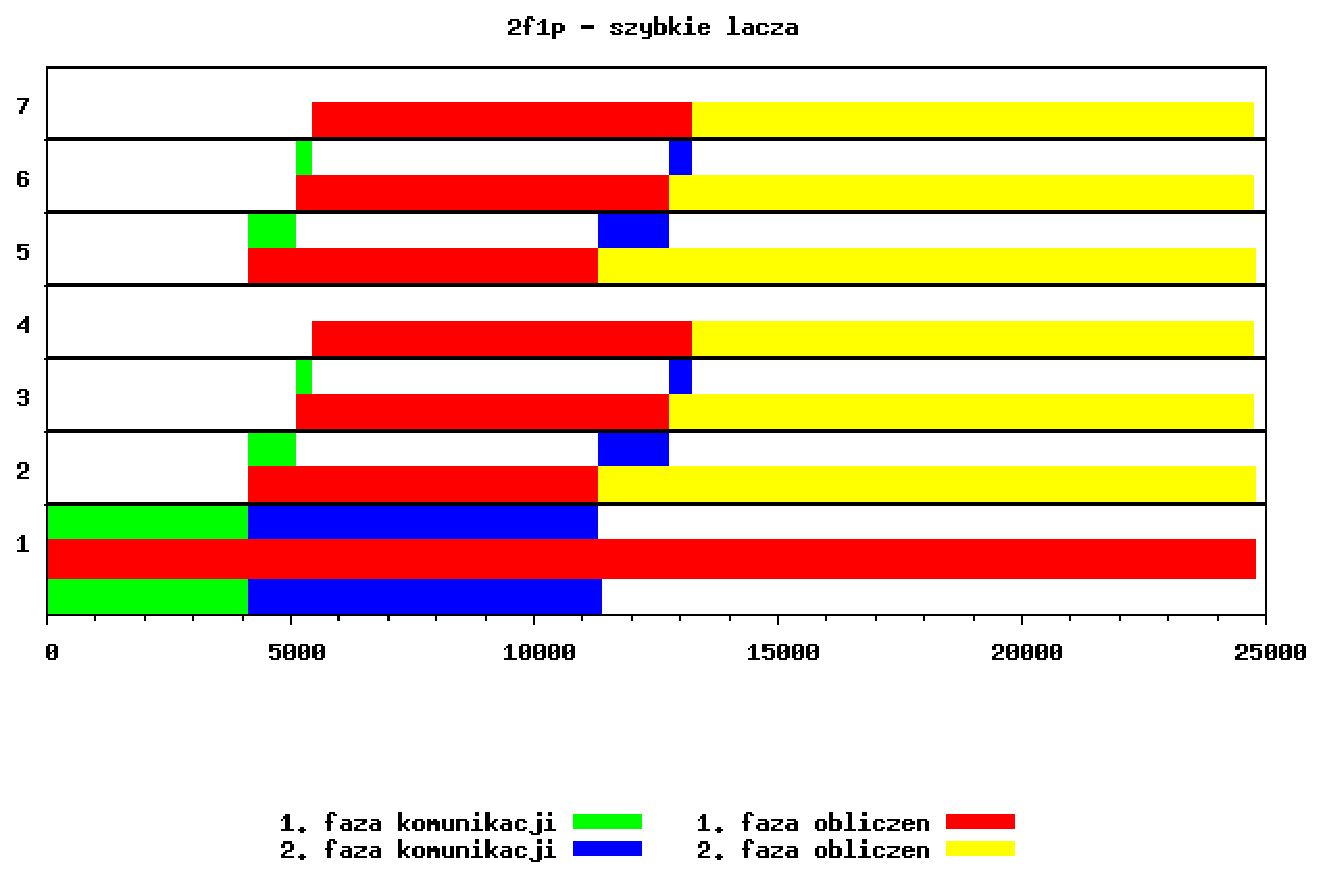
\includegraphics[width=1.0\textwidth]{wykresy/1p2f_lacza}
\caption{Diagram Gantta dla modelu 2f1p z maksymalizacją szybkich łączy \label{1p2f_l}}
\end{figure}

\section{Opis implementacji modeli}
Zaimplementowano programy realizujące modele 1f1p oraz 1f2p w wersjach uwzględniających architekturę zarówno dla maksymalizacji liczby szybkich procesorów jak i maksymalizacji liczby szybkich łączy - patrz opis zadania. Dla każdego transputera użytego w danej implementacji stworzono dwa procesy: obliczeniowy i pomiarowo-komunikacyjny. Proces obliczeniowy uruchamiano z priorytetem niskim. Natomiast proces pomiarowo-komunikacyjny z priorytetem wysokim.

Pierwszą fazą działania programów była synchronizacja porcesów. Po dokonaniu synchronizacji na każdym z transputerów, począwszy od najbardziej zewnętrznych, odczytywano aktualną wartość zegara, następnie przesyłano komunikat w kierunku środka łańcucha. Każdy następny transputer odbierając ten komunikat pobierał aktualną wartość TimeProc(). Pomierzone w ten sposób czasy uznano za początek przetwarzania. Jako, że najpierw mierzono czas na najbardziej zewnętrznych transputerach, należy mieć na uwadze, że uzyskane na nich względne punkty pomiarowe (liczone od rozpoczęcia przetwarzania) są nieco większe od faktycznych. Różnica ta jest niewielka w stosunku do długości operacji na danych.

\subsection{Model 1f1p}
W modelu tym mierzono trzy momenty czasowe dla każdego z transputerów: bezpośrednio przed i po wyslaniu danych do kolejnego transputera oraz po otrzymaniu informacji o zakończeniu obliczeń. Do rozsyłania danych z centralnego transputera użyto dwóch procesów o wysokim priorytecie realizujących zadanie równocześnie. Obliczenia wykonywano na procesach o niskim priorytecie, co gwarantowało, że będą one uruchamiane w czasie wysyłania danych, nie blokując jednocześnie inicjalizacji tego wysyłania. Gdy proces komunikacyjny otrzymał dane, wysyłał informację synchronizującą do procesu obliczeniowego, informując o możliwości rozpoczęcia obliczeń. Następnie proces o wysokim priorytecie inicjował przesyłanie danych na kolejny transputer. Po zakończeniu przetwarzania proces o niskim priorytecie wysyłał komunikat do procesu o wysokim priorytecie, na którym mierzony był czas zakończenia obliczeń. Dopiero po ustaleniu wszystkich potrzebnych czasów dane przesyłane były do procesu wejścia-wyjścia.
\subsection{Model 2f1p}
W tym  przypadku wyznaczano czasy:
\begin{itemize}
\item zakończenia odbierania pierwszej porcji danych (początku obliczeń)
\item zakończenia odbierania drugiej porcji danych (początku przesyłania danych na kolejny transputer)
\item zakończenia przesyłania pierwszej porcji danych
\item zakończenia przesyłania drugiej porcji danych
\item zakończenia obliczeń na transputerze
\end{itemize}
Struktura i zadania procesów pozostały niezmienione w stosunku do implementacj modelu 1f1p. Po otrzymaniu pierwszej porcji danych proces komunikacyjny wysyłał komunikat do procesu obliczeniowego o możliwości rozpoczęcia obliczeń, po czym odbierał drugą porcję danych, przekazując ją w dwóch porcjach do następnego transputera. Pomiar czasu zakończenia obliczeń odbywał się w sposób opisany dla modelu 1f1p.
\section{Wyniki testów implementacji dla wybranych modeli}
\subsection{Model 1f1p}
\subsubsection{Maksymalizacja liczby szybkich procesorów}
\begin{table}[hp!]
\begin{tabular}{|l|l|l|l|}\hline
transputer & poczatek przesyłania(obliczeń) & koniec przesylania & koniec obliczeń\\ \hline
1 & 0 & 10282 & 29568\\ \hline
1 & 0 & 9865  & \\ \hline
2 & 9887 & 13558 & 29189\\ \hline
3 & 13582 & 14202 & 29103\\ \hline
4 & 14224 & & 29157\\ \hline
5 & 10314 & 12370 & 29384\\ \hline
6 & 12392 & 13069 & 29448\\	\hline
7 & 13091 & & 29410\\ \hline
\end{tabular}
\caption{Wyniki pomiarów dla modelu 1f1p z maksymalizacją szybkich transputerów \label{i1f1p_p}}
\end{table}
\begin{figure}[hp!]
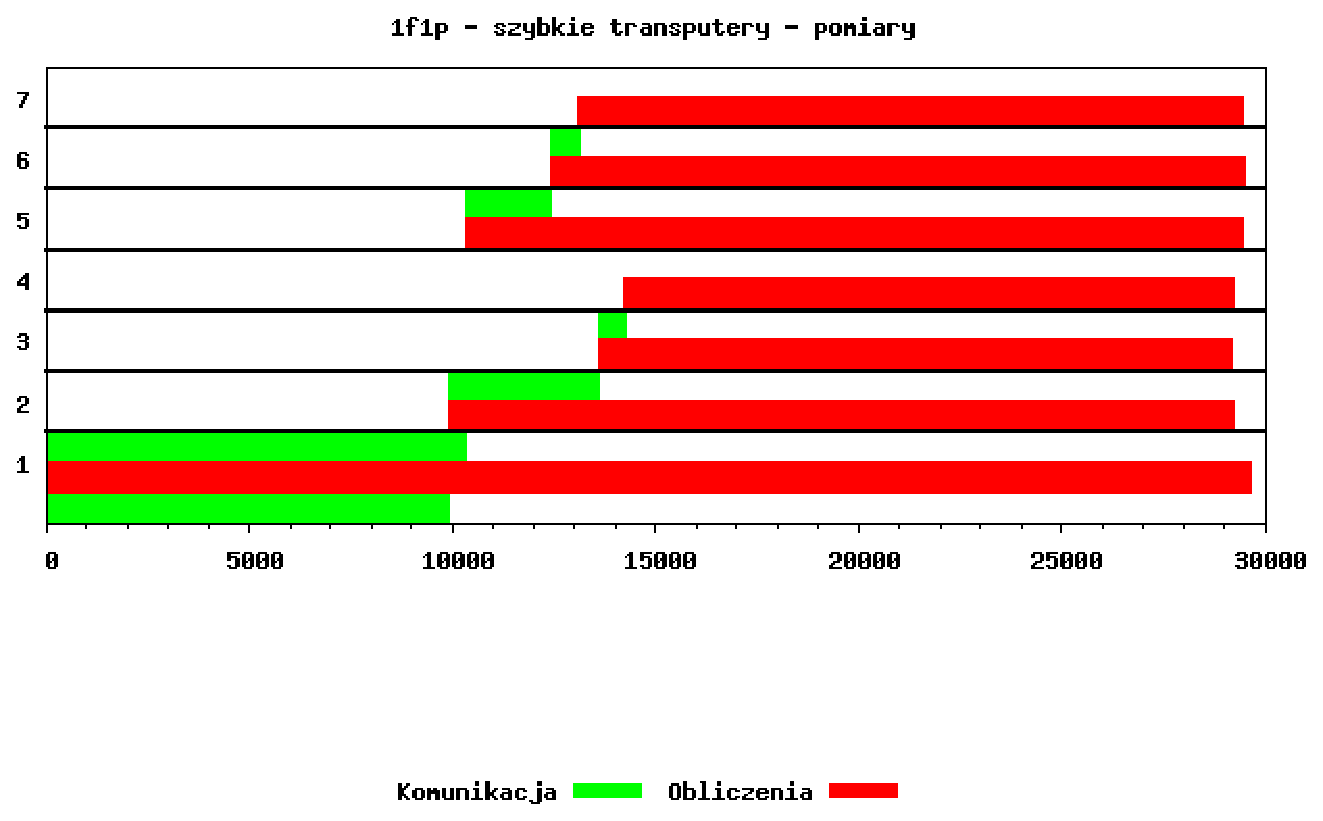
\includegraphics[width=1.0\textwidth]{wykresy/i1p1f_proc}
\caption{Diagram Gantta dla pomiarów 1f1p z maksymalizacją szybkich transputerów \label{i1p1f_pg}}
\end{figure}
\subsubsection{Maksymalizacja liczby szybkich łączy}
\begin{table}[hp!]
\begin{tabular}{|l|l|l|l|}\hline
transputer & poczatek przesyłania(obliczeń) & koniec przesylania & koniec obliczeń\\ \hline
1&0&10234&29434\\ \hline
1&0&10003&\\ \hline
2&10026&12075&29002\\ \hline
3&12098&12773&29071\\ \hline
4&12794&&29056\\ \hline
5&10265&12312&29243\\ \hline
6&12334&13010&29308\\ \hline
7&13031&&29294\\ \hline
\end{tabular}
\caption{Wyniki pomiarów dla modelu 1f1p z maksymalizacją szybkich łączy \label{i1f1p_l}}
\end{table}
\begin{figure}[hp!]
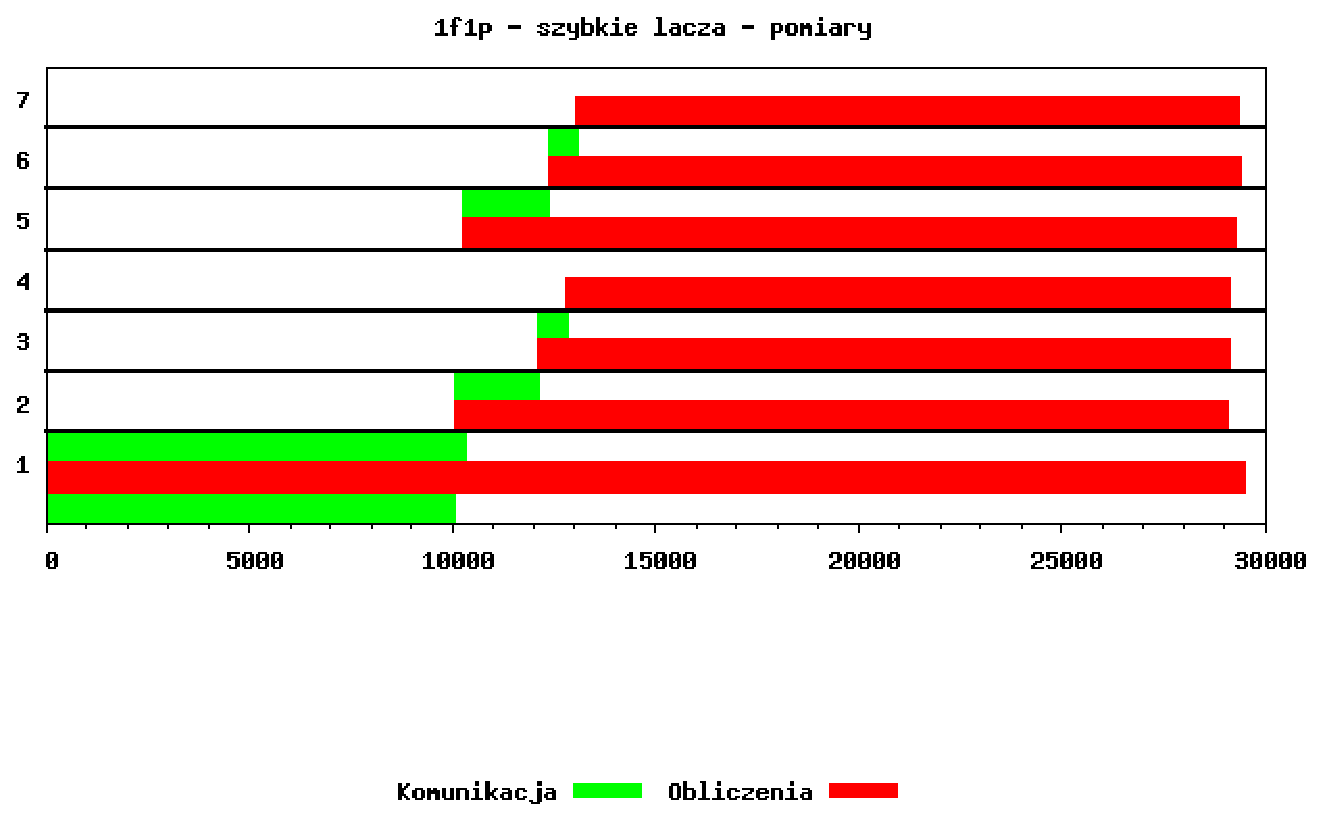
\includegraphics[width=1.0\textwidth]{wykresy/i1p1f_lacza}
\caption{Diagram Gantta dla pomiarów 1f1p z maksymalizacją szybkich łączy \label{i1p1f_lg}}
\end{figure}
\subsection{Model 1f2p}
\subsubsection{Maksymalizacja liczby szybkich procesorów}
\begin{table}[h!]
\begin{tabular}{|l|l|l|l|l|l|}\hline
Transputer&Odebranie&Odbieranie&Wysyłanie&Wysyłanie&Koniec obliczeń\\
&1. paczki&2. paczki&1. paczki&2. paczki&\\ \hline
1&0&0&7031&10395&28673\\ \hline
1&0&0&6873&10405&10405\\ \hline
2&6896&10421&12890&13969&28350\\ \hline
3&12913&13985&14553&14553&28207\\ \hline
4&14575&14575&14575&14575&28236\\ \hline
5&7061&10418&11781&12163&28468\\ \hline
6&11804&12178&12553&12553&28490\\ \hline
7&12576&12576&12576&12576&21478\\ \hline
\end{tabular}
\caption{Wyniki pomiarów dla modelu 1f2p z maksymalizacją szybkich transputerów \label{i2f1p_p}}
\end{table}
\begin{figure}[hp!]
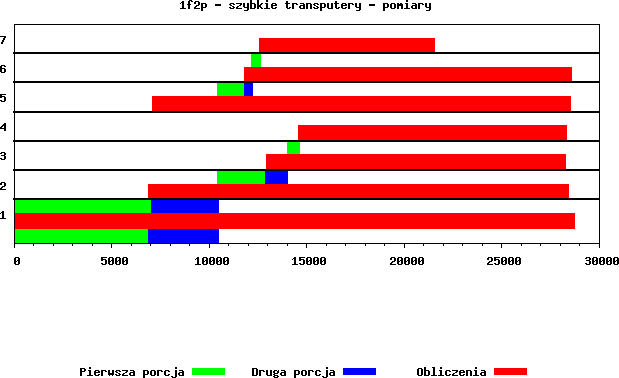
\includegraphics[width=1.0\textwidth]{wykresy/i2p1f_proc}
\caption{Diagram Gantta dla pomiarów 1f2p z maksymalizacją szybkich transputerów \label{i2p1f_pg}}
\end{figure}
\subsubsection{Maksymalizacja liczby szybkich łączy}
\begin{table}[hp!]
\begin{tabular}{|l|l|l|l|l|l|}\hline
Transputer&Odebranie&Odbieranie&Wysyłanie&Wysyłanie&Koniec obliczeń\\
&1. paczki&2. paczki&1. paczki&2. paczki&\\ \hline
1&0&0&7000&10351&28545\\ \hline
1&0&0&6842&10529&10529\\ \hline
2&6866&10546&11873&12499&28202\\ \hline
3&11895&12514&13134&13134&28153\\ \hline
4&13158&13158&13158&13158&28091\\ \hline
5&7031&10375&11733&12113&28348\\ \hline
6&11755&12127&12500&12500&28388\\ \hline
7&12523&12523&12523&12523&21371\\ \hline
\end{tabular}
\caption{Wyniki pomiarów dla modelu 1f2p z maksymalizacją szybkich łączy \label{i2f1p_l}}
\end{table}
\begin{figure}[hp!]
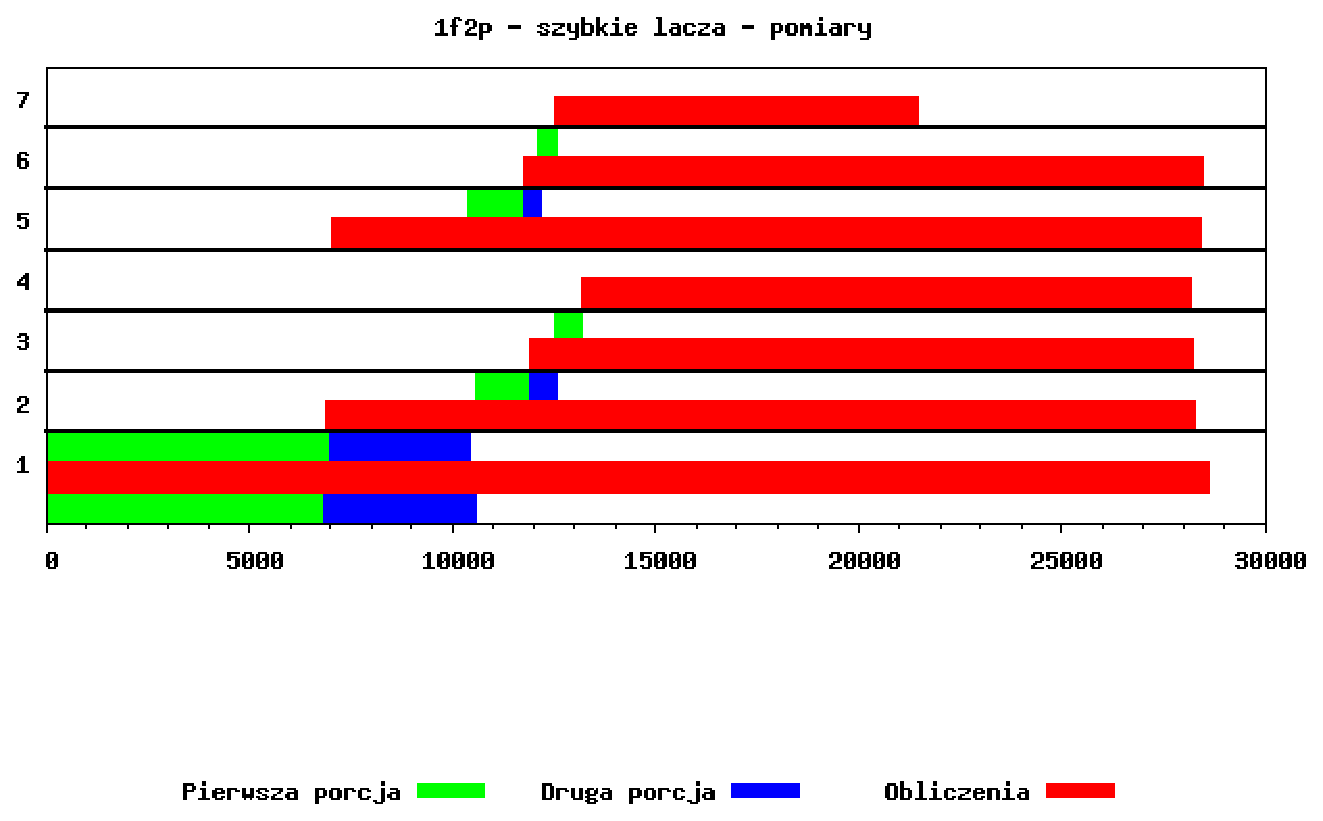
\includegraphics[width=1.0\textwidth]{wykresy/i2p1f_lacza}
\caption{Diagram Gantta dla pomiarów 1f2p z maksymalizacją szybkich łączy \label{i2p1f_lg}}
\end{figure}
\section{Porównanie wyników implementacji z wynikami uzyskanymi dla modelu teoretycznego}
\section{Wnioski}
\end{document}